\documentclass[crop, border=.1cm]{standalone}
\usepackage[utf8]{inputenc}
\usepackage{tikz}
\usepackage{amsfonts}
\usetikzlibrary{positioning, arrows.meta}

\begin{document}
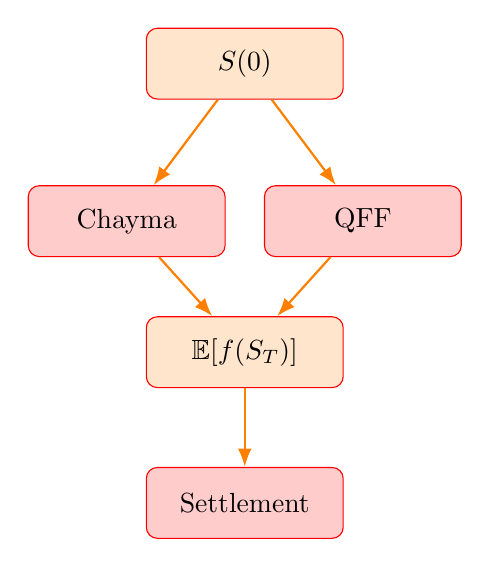
\begin{tikzpicture}[
		node distance=1.8cm and 2.5cm,
		every node/.style={draw, rounded corners, align=center, minimum width=2.5cm, minimum height=0.9cm, draw=red},
		arrow/.style={-Latex, thick, draw=orange}
	]

	% Nodes
	\node[style={fill=orange!20}] (start) {$S(0)$};
	\node[style={fill=red!20}](left) at ([xshift=-1.5cm, yshift=-2cm]start) {Chayma};
	\node[style={fill=red!20}](right) at ([xshift=1.5cm, yshift=-2cm]start) {QFF};
	\node[style={fill=orange!20}](merge) [below=2.75cm of start] {$\mathbb{E}[f(S_T)]$};
	\node[style={fill=red!20}](end) [below=1cm of merge] {Settlement};

	% Connections
	\draw[arrow] (start) -- (left);
	\draw[arrow] (start) -- (right);

	\draw[arrow] (left) -- (merge);
	\draw[arrow] (right) -- (merge);

	\draw[arrow] (merge) -- (end);

\end{tikzpicture}
\end{document}